\section{successioni}
\label{sec:successioni}

Una \emph{successione}%
\mymargin{successione}%
\index{successione} in un insieme $X$ è una
funzione $\vec a\colon \NN \to X$.
L'insieme delle funzioni $\NN \to X$ viene usualmente indicato
con $X^\NN$ e potremmo dunque scrivere $\vec a \in X^\NN$. 
In effetti una successione $\vec a$ può essere interpretata
come una sequenza infinita di elementi di $X$:
\mynote{%
Utilizziamo il grassetto per evidenziare il fatto
che $\vec a$ non è un numero ma una \emph{lista} (o vettore) di numeri.
Nella scrittura a mano non è possibile usare il grassetto, ma potremmo
sottolineare il nome della variabile scrivendo $\underline a$ invece che $\vec a$.
In alternativa si potrebbe scrivere $\stackrel{\rightarrow}a$ oppure evitare
qualunque distinzione e scrivere più semplicemente $a$.}
\[
  \vec a = (a_0, a_1, a_2, \dots, a_n, \dots )
\]
dove si intende
\[
   a_n = \vec a(n).
\]
Le componenti $a_n$ si chiamano \emph{termini} della successione.
I numeri $n$ si chiamano, invece, \emph{indici}.
L'intera
successione $\vec a$ può essere indicata con $(a_n)_{n=0}^\infty$
oppure $(a_n)_n$ oppure,
più semplicemente, con $a_n$ quando sia chiaro che si intende l'intera
successione $\vec a$ e non un singolo termine della stessa.%

Per noi il caso più interessante sarà quello delle \emph{successioni reali}
$a_n\in \RR$ cioè il caso $X=\RR$. Considereremo però anche il caso di
\emph{successioni complesse} $a_n\in \CC$ (dunque $X=\CC$) perché questo
potrà essere utile in alcune situazioni.%
\mynote{In alcuni testi le successioni vengono indicate
con la notazione $\ENCLOSE{a_n}$ che però è fuorviante in quanto
una successione in $X$ non è semplicemente un sottoinsieme di $X$:
l'ordine in cui vengono presi gli elementi è rilevante.}

\subsection{limite di successione}

Visto che $\vec a \colon \NN\to\RR$ (o in $\CC$) è una funzione 
con dominio $\NN\subset \RR$ 
e visto che $+\infty$ è l'unico punto di accumulazione di $\NN$ 
sarà possibile considerare il limite
\[
  \ell = \lim_{n\to +\infty} \vec a(n)
\]
che potremmo anche scrivere con una delle seguenti notazioni:
\[
\ell = \lim \vec a = \lim_n a_n = \lim_{n\to +\infty} a_n
\]
o più concisamente:
\[
  a_n \to \ell. 
\]

Esplicitando la definizione astratta di limite osserviamo che se $(\alpha,+\infty]$
è un intorno di $+\infty$ con $\alpha>0$ la sua intersezione con $\NN$ (il dominio della funzione)
è l'insieme $\ENCLOSE{n\in \NN\colon n> N}$ dove $N=\lfloor \alpha \rfloor$ è 
un numero naturale. Dunque se $\ell \in \RR$ 
la condizione $a_n \to \ell$ si esplicita nel modo seguente:
\begin{equation}\label{eq:limite_successione_convergente}
\forall \eps>0\colon \exists N\in \NN\colon n>N\implies \abs{a_n-\ell} < \eps.  
\end{equation}
La condizione $a_n\to +\infty$ si scrive
\[
  \forall \alpha\in \RR \colon \exists N\in \NN \colon n>N \implies a_n > \alpha  
\]
e infine $a_n\to-\infty$ diventa
\[
  \forall \alpha\in \RR \colon \exists N\in \NN \colon n>N \implies a_n < -\alpha.    
\]

\begin{definition}[carattere di una successione]
Sia $a_n$ una successione a valori reali o complessi
e si consideri il limite 
\[
  \lim_n a_n.  
\]
Se tale limite esiste diremo che la successione $a_n$ è 
\emph{regolare}%
\mymargin{regolare}%
\index{regolare},
\index{successione!regolare}%
se il limite esiste ed è finito diremo che la successione è 
\emph{convergente}%
\mymargin{convergente}%
\index{convergente}%
\index{successione!convergente}
se il limite è infinito diremo che la successione è 
\emph{divergente}%
\mymargin{divergente}%
\index{divergente}%
\index{successione!divergente}
se il limite non esiste diremo infine che la successione è
\emph{indeterminata}%
\mymargin{indeterminata}%
\index{indeterminato}%
\index{successione!indeterminata}.

Abbiamo dunque le seguenti alternative
\begin{enumerate}
 \item la successione è convergente (ha limite finito);
 \item la successione è divergente (ha limite infinito);
 \item la successione è indeterminata (non ha limite).
\end{enumerate}
Determinare il \emph{carattere}
\mymargin{carattere di una successione}%
\index{carattere!di una successione}%
\index{successione!carattere}%
di una successione
significa specificare a quale delle tre categorie appartiene.
\end{definition}

\begin{exercise}
Una successione complessa $z_n\in \CC$ potrà essere scritta
nella forma $z_n = x_n + i y_n$ dove $x_n$ e $y_n$ sono successioni
reali. Si può allora verificare che $z_n\to z$ per $z\in \CC$ se e solo se
$x_n\to x$ e $y_n\to y$ dove $z=x+ iy$ con $x,y\in \RR$.
\end{exercise}

Si faccia attenzione al fatto che una successione $a_n\in \RR \subset \CC$
può essere interpretata sia come successione reale che come successione complessa.
Le condizioni di convergenza in $\RR$ o $\CC$ sono allora equivalenti. Ma
se $a_n \to \infty$ (in $\bar \CC$) significa che $\abs{a_n}\to +\infty$
e può capitare che $a_n$ non abbia limite né $+\infty$
né $-\infty$ in quanto potrebbe frequentemente cambiare di segno
(un esempio è $a_n = (-n)^n$).

In generale potremmo avere delle successioni definite solamente 
su un sottoinsieme $\NN$ dei numeri naturali. 
Finché la successione è definita in un intorno di $+\infty$ (cioè 
da un certo $n_0$ in poi) questo non ha nessuna conseguenza sul 
limite per $n\to +\infty$ (grazie alla località del limite, 
teorema~\ref{th:localita_limite}).

\begin{example}
  La successione $a_n = 1/n$ è definita per $n\in \NN$ ma $n\neq 0$.
  Ciò non toglie che possiamo studiarne il limite come qualunque altra
  successione. Per evidenziare il fatto che il primo indice è $n=1$
  si potrà usare la notazione $(a_n)_{n=1}^\infty$.
\end{example}
 
\subsection{successioni limitate}
\label{sec:successione_limitata}%

Se abbiamo una successione $a_n$ reale possiamo anche considerare gli operatori:
\[
  \sup_n a_n, \qquad 
  \inf_n a_n, \qquad 
  \max_n a_n, \qquad 
  \min_n a_n 
\]
che sono definiti come per qualunque altra funzione. 
Sappiamo che $\sup$ e $\inf$ esistono sempre (in $\bar\RR$) mentre $\max$ e $\min$
potrebbero non esistere.

Anche il concetto di limitatezza per una successione è ereditato dallo stesso 
concetto valido per le funzioni.
Una successione $a_n$ (a valori reali o complessi) si dice essere 
\emph{limitata}%
\mymargin{limitata}%
\index{limitato} se 
l'insieme $\{\abs{a_n}\colon n \in \NN\}$ è limitato. Cioè se 
\[
\sup_n \abs{a_n} < +\infty.  
\]
\mynote{si noti che anche quando $a_n$ è complessa la successione 
dei moduli $\abs{a_n}$ è reale (e non negativa).
Vedremo nel seguito che le successioni a valori complessi non creano 
molte più difficoltà di quanto ne creino le successioni che assumono 
valori negativi. 
Il vero vantaggio si avrà con le successioni a valori positivi, 
per questo spesso si considera il modulo di una successione.
}
In caso contrario la successione si dice essere \emph{illimitata}%
\mymargin{illimitata}%
\index{illimiatato}.
Queste definizioni si applicano tali e quali alle successioni di numeri 
complessi (rimpiazzando il valore assoluto con il modulo).

Se la successione ha valori reali potremo anche parlare di 
\emph{limitatezza superiore} quando $\sup a_n <+\infty$ 
e \emph{limitatezza inferiore} quando $\inf a_n > -\infty$.


\begin{example}
Si consideri $a_n = \frac{1}{n+1}$ definita per $n\in \NN$.
Allora
\[
  \sup a_n = \max a_n = 1, \qquad
  \inf a_n = 0, \qquad \text{non esiste }\min a_n.
\]
\end{example}
\begin{proof}
Per ogni $n \in \NN$ si ha $n+1\ge 1$ e quindi $a_n = 1/(n+1) \le 1$.
Visto poi che $a_0 = 1$ si ottiene immediatamente che $\max a_n = 1$
e di conseguenza $\sup a_n = 1$.

Per verificare che $\inf a_n = 0$ dobbiamo verificare innanzitutto
che $0$ è minorante, e questo è vero in quanto $a_n = 1/(n+1)> 0$ essendo $n+1\ge 1 \ge 0$.
Inoltre dobbiamo verificare che per ogni $\eps >0$ esiste $n\in \NN$ tale
che $a_n < 0 + \eps = \eps$. Questo succede se $1/(n+1) < \eps$ ovvero
se $n > 1/\eps -1$ ad esempio per $n=\lceil 1/\eps\rceil$.
Abbiamo dunque verificato che $\inf a_n = 0$.
Il minimo di $a_n$ non esiste perché se esistesse dovrebbe essere uguale
all'estremo inferiore cioè dovrebbe essere $0$. Ma questo è impossibile
perché per ogni $n\in \NN$ si ha $a_n = 1/(n+1)\neq 0$.
\end{proof}

Visto che l'insieme $\NN$ su cui sono definite le successioni 
ha un unico punto di accumulazione $+\infty$ se la successione 
è convergente non potrà essere illimitata, come viene espresso nel seguente.

\begin{theorem}[limitatezza delle successioni convergenti]
  \label{th:limitatezza_successione_convergente}%
\mymark{**}%
Se una successione (reale o complessa) è convergente allora è anche limitata.
Se una successione reale diverge a $+\infty$ allora è inferiormente limitata,
se diverge a $-\infty$ è superiormente limitata.
\end{theorem}
%
\begin{proof}
  Per la definizione di limite~\eqref{eq:limite_successione_convergente} 
  se $a_n\to \ell$ con $\ell$ finito sappiamo 
  che scelto $\eps=1$ dovrà esistere $N\in \NN$ tale che 
  \[
      \forall n>N\colon \abs{a_n - \ell} < 1.
  \]
  Osserviamo ora che gli indici $n$ per cui $n\le N$ sono in numero finito 
  (in effetti sono $N+1$) e quindi esiste
  \[
   M = \max_{n\le N} \abs{a_n} 
   = \max \ENCLOSE{\abs{a_0}, \abs{a_1}, \dots , \abs{a_N}}.  
  \]
  Dunque scelto $R=\max\ENCLOSE{\abs{\ell}+1,M}$ 
  se $n\le N$ si ha certamente $\abs{a_n}\le M \le R$
  e se $n>N$ si ha comunque, per disuguaglianza triangolare,
  \[
  \abs{a_n} \le \abs{a_n-\ell} + \abs{\ell} < 1+ \abs{\ell} \le R.  
  \]
  Dunque nel complesso risulta $\sup_n \abs{a_n}\le R$ e la successione 
  è limitata.

  Se $a_n\to +\infty$ per la definizione di limite 
  scelto $(0,+\infty]$ come intorno di $+\infty$ 
  deve esistere un indice $N\in \NN$ tale che se $n>N$ si ha $a_n>0$. 
  Ma allora posto $R=\min\ENCLOSE{0, a_0,\dots,a_N}$
  si avrà $a_n\ge R$ per ogni $n\in \NN$ e dunque la successione 
  risulta essere inferiormente limitata.

  Dimostrazione analoga si fa nel caso $a_n\to -\infty$.
\end{proof}


% \begin{theorem}[prodotto di limitata per infinitesima]
% \mymark{**}%
% \mymargin{prodotto limitata per infinitesima}%
\index{prodotto limitata per infinitesima}%
% Se $a_n$ è una successione limitata e $b_n\to 0$ allora
% $a_n\cdot b_n \to 0$ (il risultato vale sia per successioni reali 
% che per successioni complesse).
% \end{theorem}
% %
% \begin{proof}
%   Se $a_n$ è limitata significa che esiste $R>0$ tale che $\abs{a_n}\le R$ per
%   ogni $n\in \NN$.
%   Se $b_n\to 0$ sappiamo che anche $\abs{b_n}\to 0$, dunque
%   \[  
%     0
%     \le \abs{a_n\cdot b_n} 
%     = \abs{a_n}\cdot \abs{b_n} 
%     \le R\cdot \abs{b_n}\to R\cdot 0 = 0.
%   \]
%   Per il teorema dei due carabinieri deduciamo che $\abs{a_n\cdot b_n}\to 0$ 
%   e quindi $a_n\cdot b_n \to 0$.
% \end{proof}

\subsection{successioni monotòne}

Le definizioni~\ref{def:monotonia} si applicano alle successioni. 
Abbiamo quindi già definito cosa significa che una successione è 
crescente, decrescente, strettamente crescente, strettamente decrescente,
monotona, costante. Ad esempio, una successione $a_n$ si dice essere 
crescente se $n\ge m$ implica $a_n \ge a_m$.

La verifica della monotonia di una successione può essere però dimostrata 
più facilmente rispetto al caso generale delle funzioni in quanto 
possiamo utilizzare il principio di induzione, come mostrato 
nel seguente teorema.


\begin{theorem}[successioni monotòne]
  \mymark{***}%
Una successione $a_n$ è
\begin{enumerate}
\item \emph{crescente}: se per ogni $n\in \NN$ si ha $a_{n+1} \ge a_n$;
\item \emph{decrescente}: se per ogni $n\in \NN$ si ha $a_{n+1} \le a_n$;
\item \emph{strettamente crescente}: se per ogni $n\in \NN$ si ha $a_{n+1}>a_n$;
\item \emph{strettamente decrescente}: se per ogni $n\in \NN$ si ha
$a_{n+1}<a_n$;
\end{enumerate}
\end{theorem}
%
\begin{proof}
  Consideriamo ad esempio la prima condizione (funzione crescente).
Ovviamente se $a_n$ è crescente si ha $a_{n+1}\ge a_n$ in quanto $n+1 > n$.
Viceversa supponiamo che per ogni $n\in \NN$ si abbia $a_{n+1}\ge a_n$.  Allora
chiaramente $a_1\ge a_0$, $a_2\ge a_1 \ge a_0$, $a_3 \ge a_2 \ge a_1 \ge a_0$...
Per induzione si può quindi dimostrare che  $a_n \ge a_{n-1} \ge \dots \ge a_2
\ge a_1$.

Gli altri casi si svolgono in maniera analoga.
\end{proof}

\begin{example}
  La successione $a_n = n!$ è crescente 
  in quanto per ogni $n$ si ha $(n+1)! = (n+1)\cdot n! \ge n!$.
\end{example}

La monotònia di una successione è di estrema rilevanza in quanto,
come enunciato nel teorema seguente, le successioni monotòne sono regolari, 
cioè hanno sempre limite (finito o infinito). 
Questo teorema verrà utilizzato molte volte, in particolare quando vogliamo 
dimostrare che una successione ha limite ma non conosciamo esplicitamente il valore 
del limite. 
Il primo esempio notevole si ha nel Teorema~\ref{th:5767684} dove definiremo 
la costante di Nepero $e$ come il limite di una particolare successione crescente.

\begin{theorem}[regolarità delle successioni monotòne]
\label{th:limite_monotona}%
Le successioni monotòne sono regolari.
Più precisamente se $a_n$ è crescente allora $\lim a_n = \sup a_n$ 
mentre se $a_n$ è decrescente $\lim a_n = \inf a_n$.
\end{theorem}
\begin{proof}
In realtà questo teorema è un caso particolare del 
Teorema~\ref{th:limite_monotona} se ricordiamo che una successione 
$a_n$ non è altro che una funzione $f(n)=a_n$ definita sui numeri naturali.
E il limite a $+\infty$ è un limite sinistro.
Vista però l'importanza di questo risultato possiamo ripetere la dimostrazione 
in questo caso specifico.

Per fissare le idee supponiamo che la successione $a_n$ sia crescente e dimostriamo 
che $\lim a_n = \ell$ con $\ell=\sup a_n$.
Per la definizione di limite dobbiamo verificare che scelto un qualunque intorno $U$ 
di $\ell$ si ha definitivamente $a_n\in U$.
Dimostriamo anzi una condizione più forte e cioè che $a_n$ sta definitivamente 
in un intorno sinistro di $\ell$ cioè che per ogni $q<\ell$ esiste $N$ tale che 
per ogni $n\ge N$ si ha $a_n\in (q,\ell]$ (si noti che $\ell$ può essere finito o $+\infty$ 
e quanto abbiamo scritto vale in entrambi i casi).
Che valga $a_n\le \ell$ è ovvio in quanto $\ell=\sup a_n$ è, per definizione, un maggiorante 
di $a_n$. Inoltre $\ell$ è il minimo dei maggioranti e quindi preso 
$q<\ell$ sappiamo che $q$ non è un maggiorante ovvero deve esistere $N$ tale che 
$a_N > q$. Ma, essendo $a_n$ crescente, sappiamo che per ogni $n\ge N$ si ha 
$a_n \ge a_N >q$ e questo conclude la dimostrazione.
\end{proof}

%%%%%%%%%%%%%%%%%
%%%%%%%%%%%%%%%%%
%%%%%%%%%%%%%%%%%
%%%%%%%%%%%%%%%%%

\subsection{successioni ricorsive}

Le successioni ricorsive sono le successioni
definite per induzione (tramite il teorema~\ref{th:induzione}):
\[
 \begin{cases}
   a_0 = \alpha \\
   a_{n+1} = f(a_n).
 \end{cases}
\]
Si potrebbe affrontare ora il capitolo~\ref{ch:successioni_ricorsive}
per uno studio di questo tipo di successioni.
La prima parte di quel capitolo è infatti accessibile con le nozioni
che sono state sviluppate finora.
La seconda parte richiederà invece degli strumenti più avanzati.

\subsection{la costante di Nepero}

\begin{figure}
  \begin{center}
    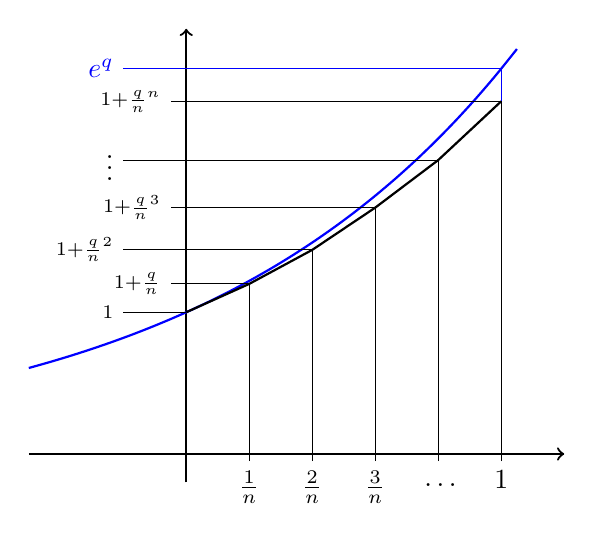
\begin{tikzpicture}[x=4.0cm,y=1.8cm]
    	\draw[thick,->] (-0.5,0) -- (1.2,0);
      \draw[thick,->] (0,-0.2) -- (0,3.0);
      %
      \draw[domain=-0.5:1.05,smooth,variable=\x,thick,blue] plot
      ({\x}, {exp(\x)});
      \draw[blue] (1.0,-0.05) -- (1.0,{exp(1.0)})
      -- (-0.2, {exp(1.0)}) node[left]{$e^q$};
      \draw (-0.2,1) node[left]{$\scriptstyle 1$} -- (0,1);
      \draw (0.2,-0.05) node[below]{$\frac 1 n$} -- (0.2,1.2)
      -- (-0.05,1.2) node[left]{$\scriptstyle 1+\frac q n$};
      \draw (0.4,-0.05) node[below]{$\frac 2 n$} -- (0.4,1.44)
      -- (-0.2,1.44) node[left]{$\scriptstyle\enclose{ 1+\frac q n}^2$};
      \draw (0.6,-0.05) node[below]{$\frac 3 n$} -- (0.6,1.738)
      -- (-0.05,1.738) node[left]{$\scriptstyle\enclose{1+\frac q n}^3$};
      \draw (0.8,-0.05) node[below]{$\rule{0mm}{2mm}\dots$} -- (0.8,2.0736)
      -- (-0.2,2.0736) node[left]{$\vdots$};
      \draw (1.0,-0.05) node [below] {$1$} -- (1.0,2.48832)
      -- (-0.05,2.48832) node[left]{$\scriptstyle\enclose{1+\frac q n}^n$};
      \draw[thick] (0,1) -- (0.2,1.2)
      -- (0.4,1.44) -- (0.6,1.738)
      -- (0.8,2.0736) -- (1.0,2.48832);
    \end{tikzpicture}
  \end{center}
  \caption{L'interesse composto.
  Se dividiamo l'intervallo $[0,1]$
  in $n$ parti (in figura $n=5$), al passo zero
  partiamo con un capitale pari ad $1$ e ad ogni
  passo di ampiezza $\frac 1 n$ moltiplichiamo
  il nostro capitale per $1+\frac q n$ (supponendo
  di avere un interesse pari a $q$ che
  nel tempo $\frac 1 n$ ci paga quindi $\frac q n$
  volte il nostro capitale).
  Dopo
  $n$ passi, cioè al tempo $1$, avremo
  un capitale pari a $\enclose{1+\frac q n}^n$.
  Se $n\to+\infty$ questa quantità tende ad $e^q$.}
  \label{fig:nepero}
\end{figure}


La funzione esponenziale è legata ad un modello di crescita che si trova spesso
in natura: la \emph{crescita esponenziale}%
\mymargin{crescita esponenziale}%
\index{crescita!esponenziale}.
Prendiamo come esempio una popolazione di batteri che cresce senza
limitazioni di spazio e di nutrimento oppure
pensiamo alla crescita di un capitale dovuto ad una rendita finanziaria.

Supponiamo che una popolazione che al tempo $t_0=0$
ammonta ad un certo numero $c$ di batteri, al tempo
$t>0$ raggiunga una numerosità $q(t,c)$.
Se lascio crescere la popolazione per un ulteriore
tempo $s>0$ troverò al tempo $t+s$ la stessa
popolazione che avrei al tempo $s$ se al tempo
zero fossi partito con la popolazione $q(t)$:
\[
  q(t+s,c) = q(s,q(t,c)).
\]
L'equazione precedente si chiama proprietà
di \emph{semigruppo}
\index{semigruppo}%
continuo.
Ma fissato $t$ la popolazione $q(t,c)$ deve
essere proporzionale a $c$ perché ogni batterio
ha la sua discendenza indipendentemente dalla numerosità
totale della popolazione. In pratica
si deve avere $q(t,c) = k(t) \cdot c$ per una opportuna
funzione $k(t)$ che non dipende da $c$.
Dunque
\[
  q(t+s,c)
  = q(s,q(t,c))
  = k(s) \cdot q(t,c)
  = k(s) \cdot k(t) \cdot c
\]
da cui
\[
  k(t+s) = k(s) \cdot k(t).
\]
In base al teorema~\ref{th:isomorfismo}
possiamo affermare
che $k(t)$ è una funzione esponenziale $k(t)=a^t$
per una qualche costante $a$.
La costante $a$ può essere determinata mediante la formula:
\[
  a = k(1) = \frac{q(1,c)}{c}
\]
ma questa espressione non ha un preciso significato fisico in quanto
dipende dall'unità di tempo scelta.

La costante a cui possiamo dare significato è invece l'aumento relativo
istantaneo della popolazione. Possiamo infatti supporre che
se lasciamo la popolazione crescere per un tempo $\Delta t$ molto piccolo,
si otterrà un aumento di popolazione proporzionale al tempo $\Delta t$
e alla popolazione:%
\mynote{stiamo qui anticipando il concetto di derivata}
\begin{equation}\label{eq:488464}
  q(\Delta t,c) = c + r c \Delta t = (1+r \Delta t) c.
\end{equation}
La costante $r$ rappresenta quindi l'aumento
relativo istantaneo della popolazione (nel caso dell'investimento
$r$ sarebbe il tasso di interesse istantaneo).
Questa definizione ha senso
quando $\Delta t$ è piccolo in quanto non tiene conto del fatto che
nell'intervallo di tempo $[t,t+\Delta t]$ la popolazione che si
è aggiunta genera anch'essa nuova popolazione (ovvero l'interesse
accumulato genera anch'esso interesse\mynote{%
In effetti la scoperta della costante $e$
è dovuta a Jacob Bernoulli (1655--1705) vedi note storiche 
a pag~\pageref{note:Bernoulli}}).

Per calcolare l'aumento della popolazione su tempi ``grandi'' possiamo
suddividere gli intervalli temporali in $n$ intervallini di ampiezza
$\Delta t$ e applicare in ognuno di essi la relazione \eqref{eq:488464}.
Si trova:
\begin{align*}
 q(\Delta t,c) &= c(1+r\Delta t) \\
 q(2\Delta t,c) &= q(\Delta t,c) (1+r\Delta t)  = c(1+r\Delta t)^2\\
 &\vdots \\
 q(n\Delta t) &= c(1+r\Delta t)^n.
\end{align*}
Dunque, ponendo $\Delta t=t/n$ si ha
\[
  q(t,c) = c\enclose{1+r\frac{t}{n}}^n
\]
in particolare per $t=1/r$ si ottiene:
\[
  q(1/r,c) = c\enclose{1+\frac{1}{n}}^n
\]
e ricordando che $q(t,c)=c a^t$ otteniamo:
\[
  a^{\frac 1 r} = \enclose{1+\frac{1}{n}}^n.
\]
Se per $n\to +\infty$ (che corrisponde a $\Delta t \to 0$)
la quantità sul lato destro tende ad un numero $e$ (che chiameremo costante
di Nepero) avremo allora
\[
  a = e^r, \qquad q(t,c) = c e^{rt}
\]
che è la relazione che lega le due costanti $a$ e $r$ che definiscono
la crescita esponenziale.

Risulta in effetti valido il seguente.

\begin{theorem}[costante di Nepero]
\mymark{**}%
\label{th:5767684}
La successione
\[
  a_n = \enclose{1+\frac 1 n}^n
\]
è crescente e limitata, dunque è convergente.
\end{theorem}
%
Per dimostrare il teorema precedente ci serve 
preliminarmente il seguente risultato.
%
\begin{theorem}[disuguaglianza di Bernoulli]
  \label{th:disuguaglianza_bernoulli}%
  \mymark{**}%
  \mymargin{disuguaglianza di Bernoulli}%
  \index{Bernoulli!disuguaglianza di}%
  \index{disuguaglianza!di Bernoulli}%
  Se $x > -1$ e $n\in \NN$ si ha
  \begin{equation}
  \label{eq:bernoulli}
  (1+x)^n \ge 1 + nx.
  \end{equation}
  \end{theorem}
  %
  \begin{proof}
  \mymark{**}
  Dimostriamo che vale~\eqref{eq:bernoulli}
  per induzione su $n$.
  Per $n=0$ la disequazione \eqref{eq:bernoulli} diventa $1\ge 1$
  ed è quindi verificata.
  Se~\eqref{eq:bernoulli}
  è verificata per un certo $n$
  moltiplicando ambo i membri per $1+x > 0$ si ottiene
  \[
  (1+x)^{n+1} \ge (1+x) (1+nx) = 1 + (n+1)x + n x^2
  \ge 1 + (n+1)x
  \]
  che è proprio la disuguaglianza~\eqref{eq:bernoulli}
  con $n+1$ al posto di $n$.
  \end{proof}
%
\begin{proof}[Dimostrazione del teorema~\ref{th:5767684}]
Dimostriamo innanzitutto che $a_n$ è crescente, cioè che
per ogni $n\ge 2$ si ha $a_n \ge a_{n-1}$.
E' chiaro che $a_n>0$ per ogni $n$,
quindi ci riconduciamo a
verificare che $\frac{a_n}{a_{n-1}} \ge 1$.

Si ha
\begin{align*}
\frac{a_n}{a_{n-1}}
&= \frac{\enclose{1+\frac 1 n}^n}{\enclose{1+\frac 1 {n-1}}^{n-1}}
= \frac{\enclose{\frac{n+1}{n}}^n}{\enclose{\frac{n}{n-1}}^{n-1}}\\
&= \enclose{\frac{n+1}{n}\cdot\frac{n-1}{n}}^n \cdot \frac{n}{n-1}
= \enclose{\frac{n^2- 1}{n^2}}^n \cdot \frac{n}{n-1}
\end{align*}
Osserviamo ora che la disuguaglianza di Bernoulli, 
teorema~\ref{th:disuguaglianza_bernoulli},
garantisce
\[
  \enclose{\frac{n^2 -1}{n^2}}^n
  = \enclose{1-\frac{1}{n^2}}^n
  \ge 1 - \frac{n}{n^2} = 1 - \frac{1}{n} = \frac{n-1}{n}
\]
da cui si ottiene, come volevamo, $a_n / a_{n-1} \ge 1$ cioè
$a_n$ è crescente.

Se ora consideriamo la successione
\[
  b_n = \enclose{1+\frac 1 n}^{n+1}
\]
osserviamo che si ha
\[
  b_n = \enclose{1+\frac 1 n}^n \cdot \enclose{1+\frac 1 n}
   = a_n\cdot \enclose{1+\frac 1 n} > a_n.
\]
Per dimostrare che $a_n$ è limitata sarà quindi sufficiente dimostrare
che $b_n$ è superiormente limitata. Vedremo ora che $b_n$ è decrescente (e quindi $a_n \le b_n \le b_1$ è superiormente limitata).

Procediamo in maniera analoga a quanto fatto per $a_n$:
\begin{align*}
\frac{b_{n-1}}{b_n}
& = \frac{\enclose{1+\frac{1}{n-1}}^n}{\enclose{1+\frac{1}{n}}^{n+1}}
  = \frac{\enclose{\frac{n}{n-1}}^n}{\enclose{\frac{n+1}{n}}^{n+1}}
  = \enclose{\frac{n}{n-1}\cdot\frac{n}{n+1}}^{n+1}\cdot\frac{n-1}{n} \\
& = \enclose{\frac{n^2}{n^2-1}}^{n+1} \cdot \frac{n-1}{n}
  = \enclose{1 + \frac{1}{n^2-1}}^{n+1} \cdot \frac{n-1}{n}.
\end{align*}
In base alla disuguaglianza di Bernoulli otteniamo
\[
  \enclose{1 + \frac{1}{n^2-1}}^{n+1}
  \ge 1 + (n+1) \cdot \frac{1}{n^2-1}
  = 1 + \frac{1}{n-1} = \frac{n}{n-1}.
\]
Mettendo insieme le due stime si ottiene dunque $b_{n-1}/b_n \ge 1$
che è quanto ci rimaneva da dimostrare.
\end{proof}

E' quindi giustificata la seguente.

\begin{definition}[costante di Nepero]
\mymark{***}
Definiamo la \emph{costante di Nepero}%
\mymargin{costante di Nepero}%
\index{costante!di Nepero}%
\index{$e$}%
\mynote{John Napier (1550-1617) vedi note storiche a pag~\pageref{nota:Nepero}}%
\[
  e = \lim_{n\to +\infty} \enclose{1+\frac 1 n}^n,
  \qquad n\in\NN.
\]
\end{definition}

Sapendo che
\[
  \enclose{1+\frac 1 n}^n \le e \le \enclose{1+\frac 1 n}^{n+1}
\]
e ponendo $n=1$ otteniamo $2\le e \le 4$.

\begin{exercise}\label{ex:4876765}
Posto $a_n = \frac{n^n}{n!}$ mostrare che $\frac{a_{n+1}}{a_n} \to e$.
\end{exercise}


\begin{theorem}[limiti che si riconducono al numero $e$]
\mymargin{limiti che si riconducono al numero $e$}%
\index{limiti che si riconducono al numero $e$}
Si ha 
\[
\lim_{x\to 0}  \enclose{1 + x}^{\frac 1 {x}} = e.
\]
\end{theorem}
%
\begin{proof}
  Iniziamo col dimostrare che 
  \begin{equation}\label{eq:2373793}
    \lim_{x\to +\infty} \enclose{1+\frac 1 x}^x = e.
  \end{equation}
  Ogni numero reale $x$ è compreso tra due interi consecutivi:
  \[
      \lfloor x \rfloor \le x \le \lfloor x\rfloor + 1
  \]
  e dunque
  \[
    1+\frac{1}{\lfloor x\rfloor +1 } 
    \le 1 + \frac 1 x 
    \le 1 + \frac 1 {\lfloor x\rfloor} 
  \]
  da cui 
  \begin{equation}\label{eq:48675248}
    \enclose{1+\frac{1}{\lfloor x\rfloor +1 }}^{\lfloor x\rfloor} 
    \le \enclose{1 + \frac 1 x }^x
    \le \enclose{1 + \frac 1 {\lfloor x\rfloor}}^{\lfloor x\rfloor +1}. 
  \end{equation}
  Per calcolare il limite della espressione a sinistra 
  operiamo il cambio di variabile $n=\lfloor x\rfloor + 1$ per 
  ottenere:
  \begin{align*}
  \lim_{x\to+\infty} \enclose{1+\frac{1}{\lfloor x\rfloor +1 }}^{\lfloor x\rfloor}
  &= \lim_{n\to +\infty} \enclose{1+\frac 1 n}^{n-1}\\
  &= \lim_{n\to +\infty} \frac{\enclose{1+\frac 1 n}^{n}}{1+\frac 1 n}
   = \frac{e}{1} = e.
  \end{align*}
  Similmente per quanto riguarda il limite della espressione a destra 
  si può operare il cambio di variabile $n=\lfloor x\rfloor$:
  \begin{align*}
    \enclose{1 + \frac 1 {\lfloor x\rfloor}}^{\lfloor x\rfloor +1}
    &= \lim_{n\to+\infty} \enclose{1+\frac 1 n}^{n+1} \\
    &= \lim_{n\to+\infty} \enclose{1+\frac 1 n}^n 
    \cdot \enclose{1 + \frac 1 n} 
    = e \cdot 1 = e.
  \end{align*}
  Dunque per il teorema dei due carabinieri otteniamo
  che anche l'espressione 
  al centro in~\eqref{eq:48675248} tende ad $e$.
  Come conseguenza, tramite il cambio di variabile $x\mapsto \frac 1 x$
  si ottiene 
  \[
  \lim_{x\to 0^+}\enclose{1+x}^{\frac 1 x} = e.  
  \]

  Consideriamo ora il limite per $x\to -\infty$ 
  della solita espressione. 
  Tramite il cambio di variabile $y=-x$ si ha 
  \begin{align*}
  \lim_{x\to -\infty} \enclose{1+\frac{1}{x}}^x 
  &= \lim_{y\to +\infty} \enclose{1 - \frac 1 y}^{-y}
   = \lim_{y\to +\infty} \enclose{\frac {y-1} y}^{-y}\\
  &= \lim_{y\to +\infty} \enclose{\frac{y}{y-1}}^y
   = \lim_{y\to +\infty} \enclose{1 + \frac{1}{y-1}}^y\\
  &= \lim_{y\to +\infty} \enclose{1 + \frac{1}{y-1}}^{y-1}
    \cdot\enclose{1+\frac 1 {y-1}} 
    = e\cdot 1 = e.\\
  \end{align*}
  Di conseguenza, facendo il cambio di variabile $x\mapsto \frac 1 x$ 
  si ottiene
  \[
  \lim_{x\to 0^-} \enclose{1+x}^{\frac 1 x} = e.
  \]
  Mettendo insieme limite destro e limite sinistro si ottiene 
  infine il limite completo per $x\to 0$. 
\end{proof}
%
\begin{corollary}%
\label{cor:limite_notevole_ex}%
\mymark{**}%
Per ogni $x\in \RR$ si ha
\[
  \lim_{n\to +\infty} \enclose{1+ \frac x n}^n = e^x.
\]
\end{corollary}
%
\begin{proof}
Infatti, per il teorema precedente, posto $y = x/n$ si ha
$y\to 0$ per $n\to +\infty$ e quindi
\[
\lim_{n\to +\infty}\enclose{1+\frac x n}^{\frac n x} 
= \lim_{y\to 0} \enclose{1+y}^{\frac 1 y}
= e.
\]
Ma allora
\[
\enclose{1+ \frac x n}^n = \enclose{\enclose{1+\frac x n}^{\frac n x}}^x
\to e^x
\]
\end{proof}

\begin{definition}[logaritmi naturali]
Vedremo che il numero $e$ risulta essere una base naturale per la funzione
esponenziale e di conseguenza per il logaritmo. Il logaritmo in base
$e$ viene chiamato \emph{logaritmo naturale}%
\mymargin{logaritmo naturale}%
\index{logaritmo!naturale} e viene indicato con $\ln = \log_e$.
\end{definition}

\mynote{%
In alcuni testi si utilizza l'operatore $\log$, indicato senza una base esplicita,
ma la definizione non è completamente condivisa.
In certi testi (per lo più in ambito matematico)
si definisce $\log  = \ln = \log_e$,
in altri testi si considera $\log = \log_{10}$.
}

\begin{corollary}[limiti notevoli]\label{cor:limite_notevole_e}
\mymark{*}%
Si ha
\begin{gather}
 \lim_{x\to 0} \frac{\ln \enclose{1+ x}}{x} = 1; \\
 \lim_{x\to 0} \frac{e^x-1}{x} = 1.
\end{gather}
\end{corollary}
%
\begin{proof}
Per quanto riguarda il logaritmo ci si riconduce al teorema precedente
osservando che:
\[
  \frac{\ln(1+x)}{x}
  = \ln \enclose{(1+x)^{\frac 1 {x}}}
  \to \ln e = 1.
\]
Per l'esponenziale ci si riconduce al logaritmo
osservando che posto
\[
  y = e^x-1
\]
se $x\to 0$ anche $y\to 0$ e quindi si ha:
\[
\frac{e^{x}-1}{x} = \frac{y}{\ln(1+y)} \to 1.
\]

\end{proof}

\begin{exercise}
Mostrare che
\begin{gather*}
  \lim_{n\to+\infty} n^n\cdot \enclose{\frac{n+1}{n^2+1}}^n = e; \\
  \lim_{n\to+\infty} n\cdot \ln\enclose{1 + \frac 1 n} = 1; \\
  \lim_{n\to+\infty} \enclose{1-\frac{n+1}{n!}}^{(n-1)!} = \frac 1 e; \\
  \lim_{n\to+\infty} n \cdot \enclose{\sqrt[n]{2}-1} = \ln 2.
\end{gather*}
\end{exercise}

%%%%%%%%%%%%%%%%%%%
%%%%%%%%%%%%%%%%%%%
%%%%%%%%%%%%%%%%%%%
%%%%%%%%%%%%%%%%%%%
\subsection{criteri del rapporto e della radice}

Succede spesso di dover determinare il limite
del rapporto di due successioni che tendono entrambe a infinito
oppure entrambe a zero.
In queste situazioni il teorema del limite del rapporto non
si applica in quanto siamo di fronte ad una forma indeterminata.
Dovremo quindi capire quale delle due successioni
tende a infinito o a zero ``più velocemente''.

I teoremi che seguono si basano (in maniera più o meno implicita)
sull'andamento della successione geometrica:
\[
  a_n = q^n
\]
dove $q>0$ è una costante fissata.
Dalle proprietà della funzione esponenziale 
sappiamo che se $q>1$ si ha $q^n\to \infty$.
Se $q=1$ chiaramente $q^n=1\to 1$
e se $q<1$ si ha $q^{-1}>1$ e quindi $q^{-n} \to +\infty$
da cui $q^n \to 0$.

\begin{theorem}[criterio del rapporto]
\label{th:criterio_rapporto}
\index{criterio!del rapporto per le successioni}
\index{rapporto!criterio del}
  Sia $a_n$ una successione reale a termini positivi
  $a_n > 0$ tale che esista il limite del rapporto di due termini consecutivi:
  \[
     \frac{a_{n+1}}{a_n} \to \ell \in [0,+\infty].
  \]
  Se $\ell < 1$ allora $a_n \to 0$, se $\ell >1$ allora $a_n \to +\infty$.
\end{theorem}
%
%
% \begin{proof}\mynote{%
%   la dimostrazione di questo teorema si potrebbe fare in maniera
%   molto simile alla dimostrazione del teorema~\ref{th:criterio_radice}
%   senza tirare in ballo il teorema~\ref{th:criterio_cesaro} che è decisamente più complesso.
%   }
% Grazie al teorema~\ref{th:criterio_cesaro} sappiamo
% che $\sqrt[n]{a_n}\to \ell$ e quindi il risultato
% segue direttametne dal teorema~\ref{th:criterio_radice}.
% \end{proof}
%

\begin{proof}
Supponiamo sia $\ell<1$. Posto $q=(1+\ell)/2$ si ha $\ell < q < 1$ 
e posto $\eps=q-\ell>0$ per la definizione di limite $\frac{a_{n+1}}{a_n}\to \ell$ 
dovrà esistere un $N\in \NN$ tale
che per ogni $n\ge N$ si abbia:
\[
  \frac{a_{n+1}}{a_n} < \ell + \eps = q
\]
ovvero $a_{n+1} < q \cdot a_n$. In particolare si avrà:
\begin{align*}
  a_{N+1} &< q \cdot a_N \\
  a_{N+2} &< q \cdot a_{N+1} < q^2\cdot a_N \\
  a_{N+3} &< q \cdot a_{N+2} < q^3\cdot a_N \\
  \vdots
\end{align*}
ed è chiaro che per induzione potremo dimostrare che per
ogni $k\in \NN$ si ha
\[
  a_{N+k} < q^k\cdot a_N.
\]
Osserviamo però che $q^k \cdot a_N \to 0$ per $k\to +\infty$
in quanto $q<1$ e quindi $q^k \to 0$. 
Dunque, tolti i primi $N$ termini, la successione $a_n$ tende a zero. 
Ma i primi $N$ termini non influenzano né il carattere né il limite 
della successione e quindi l'intera successione $a_n$ tende a zero.

Il caso $\ell>1$ si fa in maniera analoga. Si sceglie $q$ tale
che $1<q<\ell$ e si trova, in maniera analoga al caso precedente,
che per un certo $N\in \NN$ e per ogni $k\in \NN$ si ha
\[
  a_{N+k} > q^k \cdot a_N \to +\infty.
\]
\end{proof}

Osserviamo che, nel teorema precedente (ma anche nel criterio della radice teorema~\ref{th:criterio_radice}),
non si può concludere alcunché nel
caso in cui sia $\ell = 1$.
Ad esempio le due successioni $a_n = 1/n$ e $b_n = n$
hanno limiti diversi ($a_n \to 0$, $b_n\to +\infty$) ma per entrambe
il limite del rapporto di termini consecutivi tende ad $\ell=1$.

\begin{exercise}
Mostrare che
\begin{gather*}
  \lim \frac{n!}{n^n} = 0 \\
  \lim \frac{(2n)!}{(2n)^n} = +\infty
\end{gather*}
\end{exercise}

\begin{theorem}[criterio della radice]
\label{th:criterio_radice}%
\mymark{***}%
\mymargin{criterio della radice}%
\index{criterio!della radice per successioni}%
Sia $a_n$ una successione a termini non negativi, $a_n\ge 0$, tale che
\[
  \sqrt[n]{a_n} \to \ell
\]
con $\ell \in \bar \RR$.
Allora se $\ell<1$ si ha $a_n \to 0$ se invece $\ell > 1$ si ha $a_n \to +\infty$.
\end{theorem}
%
\begin{comment}
\begin{proof}
\mymark{**}
Consideriamo prima il caso $\ell < 1$.
Se $\lim \sqrt[n]{a_n} = \ell$ significa che per ogni $\eps>0$ la successione
$\sqrt[n]{a_n}$ risulta definitivamente minore di $\ell +\eps$.
Scegliendo opportunamente $\eps$ (ad esempio $\eps = (1-\ell)/2$) si potrà
avere $q = \ell+\eps < 1$. Dunque avremo definitivamente $\sqrt[n]{a_n}< q$
ovvero $a_n < q^n$. Per ipotesi $a_n\ge 0$
e quindi, tolto un numero finito di termini, si ottiene $0 \le a_n < q^n \to 0$
da cui $a_n \to 0$ (in quanto l'aver tolto un numero finito di termini non
cambia né il carattere né il limite della successione).

Se $\ell>1$ si potrà procedere in maniera analoga. Esisterà $q$ con $1 < q < \ell$ tale che definitivamente $\sqrt[n]{a_n} > q$ da cui $a_n > q^n \to +\infty$.
\end{proof}
\end{comment}

\begin{proof}
  Si può osservare che
  \[
    a_n = \enclose{\sqrt[n]{a_n}}^n
     = e^{n \cdot \ln \sqrt[n]{a_n}}.
  \]
  Se $\ell <1$ allora il logaritmo tende ad un numero negativo,
  l'argomento dell'esponenziale tende a $-\infty$ e quindi l'esponenziale tende a zero.

  Se invece $\ell>1$ il logaritmo tende ad un numero positivo e quindi l'esponenziale tende a $+\infty$.
\end{proof}

%%%%%
%%%%%
